\documentclass[letterpaper]{article}
\usepackage{aaai}  % Template oficial AAAI
\usepackage{times}
\usepackage{helvet}
\usepackage{courier}
\usepackage[utf8]{inputenc}
\usepackage[T1]{fontenc}
\usepackage{amsmath,amssymb}
\usepackage{booktabs}
\usepackage{tabularx}
\usepackage{graphicx}
\usepackage{algorithm}
\usepackage{algorithmic}
\usepackage{pgfplots}
\pgfplotsset{compat=1.17}

\nocopyright
\pdfinfo{
/Title (Implementacao e Avaliacao Experimental de Estruturas de Dados para a Forja do Blibblon)
/Author (Victor Cunha Marques)
}

\title{Implementação e Avaliação Experimental de Estruturas de Dados Esparsas, Filas e Pilhas para a Forja do Blibblon}
\author{
    Victor Cunha Marques\\
    Departamento de Ciência da Computação -- Universidade Federal de Minas Gerais (UFMG)\\
    Belo Horizonte, MG, Brasil\\
    \texttt{vcm1926@ufmg.br}
}

\begin{document}
\maketitle

\begin{abstract}
Este trabalho apresenta o projeto, implementação e avaliação experimental do sistema de gerenciamento e recomendação de itens para a forja de Blibblon Trombaferro. O problema exige a representação eficiente de matrizes esparsas com migração dinâmica em tempo de execução entre três formatos: Lista Cruzada (Modo L), Vetor de Tripletas Ordenado (Modo T) e formato comprimido por linha (Modo C / CSR). O sistema gerencia encomendas via Fila FIFO, rastreia \textit{builds} via Pilha LIFO e provê consultas analíticas com ranqueamento determinístico ponderado (\textsc{Poder}, \textsc{Equilibrio} e \textsc{Sinergia}). A solução foi desenvolvida estritamente em C++11 sem o uso de containers pré-implementados da STL. A análise experimental investiga sistematicamente o ponto de virada entre representações encadeadas e contíguas, mensurando perfis de carga globais, estratégias de produto interno e o impacto da localidade espacial de referência.
\end{abstract}

\section{Introdução}
Na economia de aventuras contemporânea, a busca pela \textit{build} ótima impõe aos aventureiros a necessidade de balancear múltiplos atributos distribuídos de forma esparsa em milhares de itens potenciais. Uma matriz tradicional bidimensional de dimensões $N \times T$ incorre em um desperdício de memória proporcional a $\mathcal{O}(N \times T)$, onde a grande maioria das células é identicamente nula.

O desafio central deste trabalho consiste em projetar e implementar um sistema em C++11 capaz de manipular essa informação sob restrições rigorosas de desempenho e memória, suportando quatro classes fundamentais de operações:
\begin{enumerate}
    \item Manutenção dinâmica do catálogo de modificadores com suporte a inserção, remoção física quando o valor for zero e migração a quente entre representações;
    \item Gestão de fila de espera única para forja de encomendas em ordem de chegada (FIFO);
    \item Gerenciamento de \textit{builds} com montagem e desmontagem estritamente pela ponta mais recente (LIFO);
    \item Consultas analíticas e recomendações baseadas no ranqueamento global de métricas ponderadas, desempatadas deterministicamente.
\end{enumerate}

\section{Trabalhos Relacionados}
A literatura de Estruturas de Dados e Algoritmos aborda extensivamente o armazenamento de dados esparsos. Sedgewick e Wayne~\cite{sedgewick2011} e Cormen et al.~\cite{cormen2022} discutem a dicotomia clássica entre estruturas sequenciais e encadeadas.

No domínio de matrizes esparsas, as listas cruzadas (\textit{orthogonal lists}) destacam-se pela flexibilidade na inserção e remoção pontual sem realocações maciças, ao custo de sobrecarga de memória por ponteiros e baixa localidade de referência espacial~\cite{knuth1997}. Em contrapartida, formatos contíguos ordenados (tripletas COO e CSR) favorecem a localidade de cache e percursos sequenciais compactos, ao custo de deslocamentos $\mathcal{O}(K)$ em inserções intermediárias. Para ordenação, estudos destacam a superioridade adaptativa do \textit{Insertion Sort} em entradas quase ordenadas~\cite{cormen2022}.

\section{Métodos}
A arquitetura foi estruturada modularmente em Tipos Abstratos de Dados (TADs) independentes, respeitando a vedação terminante de bibliotecas de terceiros ou da STL (\texttt{std::vector}, \texttt{std::list}, \texttt{std::stack}, \texttt{std::queue}).

\subsection{TAD Catálogo (Matriz Esparsa)}
O \texttt{Catalogo} suporta três representações internas com interface uniforme:

\paragraph{Modo L (Lista Cruzada):} Células não nulas são instâncias de \texttt{CelulaCruzada}, contendo \texttt{item}, \texttt{atributo}, \texttt{valor}, \texttt{prox\_coluna} (mantido ordenado por atributo) e \texttt{prox\_linha} (mantido ordenado por item). Dois vetores dinâmicos de cabeças (\texttt{cabecas\_linhas} e \texttt{cabecas\_colunas}) fornecem acesso indexado direto aos inícios de cada linha e coluna. A atribuição de valor zero desencadeia a desconexão física e liberação da célula.

\paragraph{Modo T (Vetor de Tripletas Contíguo):} Células não nulas residem em memória contígua como \texttt{Tripleta \{item, atributo, valor\}}, ordenadas lexicograficamente por \texttt{(item, atributo)}. As consultas utilizam busca binária em tempo $\mathcal{O}(\log K)$, onde $K$ é o número de células não nulas.

\paragraph{Modo C (Compressed Sparse Row - CSR):} Representa a matriz comprimida por linha utilizando três vetores: \texttt{csr\_valores}, \texttt{csr\_colunas} e \texttt{csr\_linha\_ptr} (de dimensão $N+1$). Proporciona percurso de linha contíguo com custo ótimo $\mathcal{O}(k_i)$ e máxima localidade espacial.

\paragraph{Migração Dinâmica:} A migração entre os modos L, T e C ocorre a qualquer momento em tempo de execução sem perda de células, garantindo transparência operacional.

\paragraph{Tratamento de Exceções:} Foi implementada uma hierarquia baseada em \texttt{std::exception} (\texttt{ExcecaoModoInvalido}, \texttt{ExcecaoIndiceInvalido}, \texttt{ExcecaoPilhaVazia}, \texttt{ExcecaoFilaVazia}), conferindo robustez defensiva sem alterar as saídas nominais da VPL.

\paragraph{Consulta por Faixa LF (Ponto Extra):} Para a consulta \texttt{LF <id\_atributo> <min> <max>}, incorporou-se um índice de vetores ordenados por valor para cada atributo. Os extremos da faixa são localizados por busca binária em $\mathcal{O}(\log c_a)$. Quando $0 \in [\text{min}, \text{max}]$, itens sem célula explícita são considerados com valor zero em $\mathcal{O}(N)$, respeitando a ordem crescente de identificador de item.

\subsection{TADs Pilha, Fila e Vetor Dinâmico}
A \texttt{Pilha} e a \texttt{Fila} foram implementadas por encadeamento explícito simples, garantindo complexidade $\mathcal{O}(1)$ no topo e nas extremidades. Para o armazenamento dinâmico de itens, atributos e aventureiros, implementou-se o template genérico \texttt{Vetor<T>}, operando com política de duplicação geométrica de capacidade.

\subsection{Cálculo de Métricas e Recomendação Global}
\begin{itemize}
    \item \textbf{PODER:} $\sum_{a=0}^{T-1} v_i(a)$, calculado somando as células não nulas da linha $i$.
    \item \textbf{EQUILIBRIO:} $1 / (1 + \sigma_i)$, onde $\sigma_i$ é o desvio padrão populacional. Para evitar laços densos de tamanho $T$, itera-se apenas sobre as $k_i$ células não nulas somando $(v_i(a) - \mu_i)^2$, e adiciona-se diretamente $(T - k_i) \cdot \mu_i^2$ para as posições nulas.
    \item \textbf{SINERGIA:} Cosseno entre a linha do item e o vetor denso da \textit{build} do aventureiro.
\end{itemize}
Para garantir determinismo estrito, as pontuações parciais das métricas são arredondadas para 6 casas decimais antes do desempate por identificador crescente.

\section{Análise de Complexidade}
Nesta seção, estabelece-se a análise assintótica rigorosa de complexidade temporal e espacial, discriminada individualmente por Tipo Abstrato de Dados (TAD) e operação. Denotam-se: $N$ como o total de itens, $T$ o total de atributos, $K$ o número global de modificadores não nulos armazenados ($K \ll N \times T$), $k_i$ o número de modificadores não nulos do item $i$, $c_a$ o número de modificadores não nulos do atributo $a$, $B$ o número de itens na \textit{build} do aventureiro ($B = |\text{Pilha}|$) e $F$ a quantidade de encomendas na fila ($F = |\text{Fila}|$).

\subsection{TAD Catálogo (Matriz Esparsa)}
O \texttt{Catalogo} encapsula o estado matricial, variando a complexidade conforme a representação ativa:

\paragraph{Modo L (Lista Cruzada):}
\begin{itemize}
    \item \textbf{Complexidade Espacial:} Requer dois vetores dinâmicos de cabeças: \texttt{cabecas\_linhas} com capacidade $\mathcal{O}(N)$ e \texttt{cabecas\_colunas} com $\mathcal{O}(T)$. Cada célula não nula aloca uma \texttt{CelulaCruzada} contendo 3 inteiros (\texttt{item}, \texttt{atributo}, \texttt{valor}) e 2 ponteiros brutos (\texttt{prox\_coluna}, \texttt{prox\_linha}), perfazendo 32 bytes por nó em arquiteturas de 64 bits. O consumo espacial total é $\mathcal{O}(N + T + K)$ palavras, com sobrecarga estrutural de dois ponteiros por entrada não nula.
    \item \textbf{Consulta Pontual:} Localizar $(i, a)$ exige percorrer a lista encadeada da linha $i$ até encontrar o atributo $a$ ou ultrapassá-lo (por estar ordenada). No pior caso, inspeciona todos os $k_i$ nós da linha: tempo $\mathcal{O}(k_i)$ ($\mathcal{O}(1)$ no melhor caso).
    \item \textbf{Inserção ($v \neq 0$):} Demanda caminhar na linha $i$ até a coluna $a$ em tempo $\mathcal{O}(k_i)$ e na coluna $a$ até a linha $i$ em tempo $\mathcal{O}(c_a)$. Caso a célula já exista, atualiza-se o valor em $\mathcal{O}(1)$. Caso seja nova, instancia-se o nó e ajustam-se 4 ponteiros em $\mathcal{O}(1)$. O tempo total é $\mathcal{O}(k_i + c_a)$.
    \item \textbf{Remoção Física ($v = 0$):} Localiza o nó na linha $i$ e na coluna $a$ ($\mathcal{O}(k_i + c_a)$), desconecta os ponteiros bidirecionais e desaloca a memória via \texttt{delete}. Tempo total: $\mathcal{O}(k_i + c_a)$.
    \item \textbf{Percurso de Linha (\texttt{LI}):} Acessa a cabeça da linha $i$ em $\mathcal{O}(1)$ e percorre os $k_i$ ponteiros \texttt{prox\_coluna}. Tempo: $\mathcal{O}(k_i)$.
    \item \textbf{Percurso de Coluna (\texttt{LA}):} Acessa a cabeça da coluna $a$ em $\mathcal{O}(1)$ e percorre os $c_a$ nós via \texttt{prox\_linha}. Tempo: $\mathcal{O}(c_a)$.
    \item \textbf{Migração Dinâmica a partir do Modo L:} Percorre todas as listas para extrair as $K$ células ordenadas em tempo $\mathcal{O}(K + N)$, desalocando a matriz encadeada em $\mathcal{O}(K + N + T)$.
\end{itemize}

\paragraph{Modo T (Vetor de Tripletas Ordenado):}
\begin{itemize}
    \item \textbf{Complexidade Espacial:} Utiliza um único vetor contíguo de structs \texttt{Tripleta \{item, atributo, valor\}}. Cada entrada consome exatamente $3 \times \text{sizeof(int)} = 12$ bytes, isenta de ponteiros. Com duplicação geométrica, a capacidade máxima não excede $2K$. Espaço total: estritamente $\mathcal{O}(K)$ palavras, constituindo a representação de menor sobrecarga de memória por célula.
    \item \textbf{Consulta Pontual:} Como os elementos estão ordenados lexicograficamente por \texttt{(item, atributo)}, a busca binária identifica a presença do par em tempo $\mathcal{O}(\log K)$.
    \item \textbf{Inserção ($v \neq 0$ novo):} A busca binária localiza o ponto de inserção em $\mathcal{O}(\log K)$. Em seguida, para manter a contiguidade física ordenada, todos os elementos à direita devem ser deslocados uma posição para a frente, demandando tempo $\mathcal{O}(K)$. O custo amortizado de duplicação do array é $\mathcal{O}(1)$. Tempo total: $\mathcal{O}(K)$.
    \item \textbf{Remoção Física ($v = 0$):} Localiza o elemento em $\mathcal{O}(\log K)$ e desloca os elementos posteriores para a esquerda em $\mathcal{O}(K)$ para fechar a lacuna. Tempo total: $\mathcal{O}(K)$.
    \item \textbf{Percurso de Linha (\texttt{LI}):} Uma busca binária localiza a primeira ocorrência do item $i$ em $\mathcal{O}(\log K)$; em seguida, realiza-se uma leitura sequencial contígua dos $k_i$ modificadores daquele item. Tempo total: $\mathcal{O}(\log K + k_i)$.
    \item \textbf{Percurso de Coluna (\texttt{LA}):} Por estarem ordenadas prioritariamente por item, as células correspondentes a um dado atributo $a$ estão dispersas no array contíguo, exigindo varredura linear exaustiva de todas as $K$ tripletas. Tempo: $\mathcal{O}(K)$.
\end{itemize}

\paragraph{Modo C (Compressed Sparse Row - CSR, Ponto Extra):}
\begin{itemize}
    \item \textbf{Complexidade Espacial:} Armazena a matriz em três vetores contíguos: \texttt{csr\_valores} ($K$ inteiros), \texttt{csr\_colunas} ($K$ inteiros) e \texttt{csr\_linha\_ptr} ($N+1$ inteiros apontando o deslocamento inicial de cada linha). Espaço total: $\mathcal{O}(N + K)$ inteiros, aliando compacidade contígua a indexação direta por linha.
    \item \textbf{Consulta Pontual:} Os limites da linha $i$ são acessados em $\mathcal{O}(1)$ via \texttt{[csr\_linha\_ptr[i], csr\_linha\_ptr[i+1])}. A busca no intervalo contíguo de tamanho $k_i$ ocorre em $\mathcal{O}(\log k_i)$.
    \item \textbf{Inserção e Remoção Física:} Localiza o atributo na linha em $\mathcal{O}(\log k_i)$, desloca até $K$ elementos contíguos nos vetores de dados ($\mathcal{O}(K)$) e propaga o ajuste de índice em \texttt{csr\_linha\_ptr} de $i+1$ até $N$ em $\mathcal{O}(N - i) = \mathcal{O}(N)$. Tempo total: $\mathcal{O}(K + N)$.
    \item \textbf{Percurso de Linha (\texttt{LI}):} Acesso indexado imediato em $\mathcal{O}(1)$ e leitura sequencial direta de $k_i$ inteiros contíguos. Tempo: ótimo $\mathcal{O}(k_i)$ com máxima localidade de referência.
    \item \textbf{Percurso de Coluna (\texttt{LA}):} Varredura de todas as linhas inspecionando seus intervalos em tempo $\mathcal{O}(K)$.
\end{itemize}

\paragraph{Índice e Consulta por Faixa LF (Ponto Extra):}
\begin{itemize}
    \item \textbf{Complexidade Espacial:} Vetor dinâmico de tamanho $T$ referenciando arrays ordenados por valor para cada atributo contendo $c_a$ elementos. Espaço adicional: $\mathcal{O}(T + K)$.
    \item \textbf{Manutenção diante de \texttt{M}:} A cada alteração matricial, a função \texttt{atualizarIndiceValor} remove a entrada antiga por varredura ($\mathcal{O}(c_a)$) e insere o novo valor via busca binária e deslocamento contíguo ($\mathcal{O}(\log c_a + c_a) = \mathcal{O}(c_a)$).
    \item \textbf{Consulta LF:} Quando $0 \notin [\text{min}, \text{max}]$, os limites da faixa são encontrados por busca binária em $\mathcal{O}(\log c_a)$; os $M$ itens recuperados são ordenados por identificador em $\mathcal{O}(M \log M)$ (ou $\mathcal{O}(M^2)$). Quando $0 \in [\text{min}, \text{max}]$, itens nulos participam da resposta por definição do enunciado, exigindo verificar todos os $N$ itens em tempo $\mathcal{O}(N \log k_i)$ no Modo T/C ou $\mathcal{O}(N \cdot \bar{k})$ no Modo L.
\end{itemize}

\subsection{TAD Pilha}
\begin{itemize}
    \item \textbf{Complexidade Espacial:} Estruturada por encadeamento simples através de nós \texttt{No \{id\_item, proximo\}}. Para uma \textit{build} contendo $B$ itens equipados, consome exatamente $B$ nós na \textit{heap} ($16$ bytes por nó em 64 bits). Espaço total: $\mathcal{O}(B)$.
    \item \textbf{Complexidade Temporal:} Operações de inserção no topo (\texttt{empilhar}) e remoção do topo (\texttt{desempilhar}) envolvem manipulação de ponteiro único em tempo estrito $\mathcal{O}(1)$. A verificação de pertencimento (\texttt{contem}) para filtragem de candidatos na recomendação realiza percurso sequencial nos nós da pilha em tempo $\mathcal{O}(B)$ no pior caso.
\end{itemize}

\subsection{TAD Fila}
\begin{itemize}
    \item \textbf{Complexidade Espacial:} Implementada por encadeamento simples com ponteiros explícitos \texttt{primeiro} e \texttt{ultimo}, associando cada encomenda aos identificadores do aventureiro e do item. Espaço total: $\mathcal{O}(F)$, onde $F$ é a quantidade de encomendas pendentes na forja.
    \item \textbf{Complexidade Temporal:} Tanto o enfileiramento ao final (\texttt{enfileirar}) quanto o desenfileiramento na ponta inicial (\texttt{desenfileirar}) executam em tempo estritamente $\mathcal{O}(1)$, sem realocações ou varreduras intermediárias.
\end{itemize}

\subsection{TAD Vetor Dinâmico (\texttt{Vetor<T>})}
\begin{itemize}
    \item \textbf{Complexidade Espacial:} Bloco contíguo de capacidade geométrica com fator multiplicativo $2\times$, garantindo capacidade alocada delimitada por $2n$. Espaço total: $\mathcal{O}(n)$, onde $n$ é o total de elementos inseridos.
    \item \textbf{Complexidade Temporal:} Acesso indexado por operador \texttt{[]} em $\mathcal{O}(1)$ via aritmética direta de ponteiros. A inserção ao final (\texttt{adicionar}) possui complexidade de tempo amortizada $\mathcal{O}(1)$, com custo pontual de realocação $\mathcal{O}(n)$ ocorrendo apenas em potências de base 2.
\end{itemize}

\subsection{TAD Aventureiro}
\begin{itemize}
    \item \textbf{Complexidade Espacial:} Agrega identificador, nome textual, uma \texttt{Pilha} de itens equipados ($\mathcal{O}(B)$) e um vetor denso de tamanho fixo $T$ (\texttt{vetor\_modificadores}) que consolida o somatório de atributos da \textit{build}. Espaço total: $\mathcal{O}(B + T)$.
    \item \textbf{Complexidade Temporal:} Na estratégia imediata, \texttt{equipar} e \texttt{subtrairModificadores} atualizam o vetor denso somando ou subtraindo os modificadores não nulos do item manipulado em tempo $\mathcal{O}(k_i)$. Na estratégia sob demanda, o recálculo integral (\texttt{recalcularBuild}) esvazia o vetor de tamanho $T$ em $\mathcal{O}(T)$ e percorre os $B$ itens da pilha consultando suas células não nulas no catálogo, totalizando tempo $\mathcal{O}(T + \sum_{j=1}^B k_{i_j})$.
\end{itemize}

\subsection{TAD Atributo e TAD Item}
\begin{itemize}
    \item \textbf{Complexidade Espacial e Temporal:} Instanciação, consulta de identificadores e nomes textuais operam estritamente em tempo $\mathcal{O}(1)$ e espaço $\mathcal{O}(1)$ por entidade.
\end{itemize}

\subsection{Métricas e Ordenação na Consulta Q}
\paragraph{Cálculo das Métricas:}
\begin{itemize}
    \item \textbf{\textsc{Poder}:} Somatório das $k_i$ células da linha do item $i$. Tempo $\mathcal{O}(k_i)$ no Modo L e Modo C; $\mathcal{O}(\log K + k_i)$ no Modo T. Espaço auxiliar: $\mathcal{O}(1)$.
    \item \textbf{\textsc{Equilibrio}:} Calcula $\mu_i$ em $\mathcal{O}(k_i)$. O desvio padrão é computado somando $(v_i(a) - \mu_i)^2$ apenas sobre as $k_i$ células existentes e adicionando diretamente o termo fechado $(T - k_i)\mu_i^2$ em tempo $\mathcal{O}(1)$ para os atributos nulos. Tempo: $\mathcal{O}(k_i)$ (Modo L/C) e $\mathcal{O}(\log K + k_i)$ (Modo T). Espaço auxiliar: $\mathcal{O}(1)$.
    \item \textbf{\textsc{Sinergia}:} Requer o produto interno entre a linha do item e a \textit{build}.
    \begin{itemize}
        \item \textit{Estratégia Vetor Denso:} Densifica a \textit{build} em um vetor contíguo de tamanho $T$ com custo prévio único $\mathcal{O}(T)$. Cada produto interno com os $N$ itens percorre apenas suas $k_i$ células com acesso indexado $\mathcal{O}(1)$ à \textit{build}. Custo total para os $N$ itens: $\mathcal{O}(T + N \cdot \bar{k})$. Espaço auxiliar: $\mathcal{O}(T)$.
        \item \textit{Estratégia Intercalação de Listas:} Intercala as células não nulas do item ($k_i$) com a lista esparsa da \textit{build} ($k_b$) sob demanda. Custo total para os $N$ itens: $\mathcal{O}(N \cdot (\bar{k} + k_b))$. Espaço auxiliar: $\mathcal{O}(1)$.
    \end{itemize}
\end{itemize}

\paragraph{Algoritmos de Ordenação para os $N$ Itens:}
\begin{itemize}
    \item \textbf{Insertion Sort:} Opera \textit{in-place}. Em dados quase ordenados (poucas modificações matriciais entre consultas consecutivas), executa em tempo linear ótimo $\mathcal{O}(N)$ com $\mathcal{O}(N)$ comparações. No pior caso (catálogo totalmente desordenado), atinge tempo quadrático $\mathcal{O}(N^2)$. Espaço auxiliar: $\mathcal{O}(1)$.
    \item \textbf{Quick Sort:} Particionamento recursivo com tempo médio $\mathcal{O}(N \log N)$ e fator constante reduzido. Pior caso $\mathcal{O}(N^2)$ minimizado por particionamento estável. Espaço auxiliar recursivo: $\mathcal{O}(\log N)$.
    \item \textbf{Merge Sort:} Divisão balanceada e intercalação determinística com tempo garantido $\mathcal{O}(N \log N)$ em todos os cenários (melhor, médio e pior caso). Espaço auxiliar: $\mathcal{O}(N)$ para vetores temporários de fusão.
\end{itemize}

\paragraph{Custo Global da Consulta Q:}
Para $m$ métricas avaliadas:
\begin{enumerate}
    \item Cálculo das métricas para os $N$ itens: $m \times \mathcal{O}(N \cdot \bar{k})$;
    \item $m$ ordenações completas de $N$ itens: $m \times \mathcal{O}(N \log N)$ (ou $m \times \mathcal{O}(N)$ em regime quase ordenado com \textit{Insertion Sort});
    \item Acumulação ponderada de pontos: $m \times \mathcal{O}(N)$;
    \item Filtragem dos itens equipados na \textit{build} de tamanho $B$: $\mathcal{O}(N \cdot B)$ comparações via \texttt{possuiItemEquipado};
    \item Ordenação final dos candidatos e seleção dos $n$ melhores: $\mathcal{O}(N \log N)$.
\end{enumerate}
O tempo global da consulta \texttt{Q} é $\mathcal{O}(m \cdot N \cdot (\bar{k} + \log N) + N \cdot B)$, com espaço auxiliar total limitado a $\mathcal{O}(N + T)$.

\begin{table*}[t]
\centering
\footnotesize
\setlength{\tabcolsep}{4.5pt}
\begin{tabularx}{\textwidth}{@{} l c c c X @{}}
\toprule
\textbf{Operação / Estrutura} & \textbf{Modo L (Lista Cruzada)} & \textbf{Modo T (Tripletas)} & \textbf{Modo C (CSR)} & \textbf{Complexidade Espacial} \\
\midrule
\multicolumn{5}{@{}l}{\textit{\textbf{TAD Catálogo (Matriz Esparsa)}}} \\
\addlinespace[2pt]
Consulta Pontual $(i, a)$ & $\mathcal{O}(k_i)$ & $\mathcal{O}(\log K)$ & $\mathcal{O}(\log k_i)$ & $\mathcal{O}(1)$ aux. \\
Inserção / Atualização ($v \neq 0$) & $\mathcal{O}(k_i + c_a)$ & $\mathcal{O}(\log K + K)$ & $\mathcal{O}(\log k_i + K)$ & $\mathcal{O}(1)$ aux. \\
Remoção Física ($v = 0$) & $\mathcal{O}(k_i + c_a)$ & $\mathcal{O}(\log K + K)$ & $\mathcal{O}(\log k_i + K)$ & $\mathcal{O}(1)$ aux. \\
Percurso de Linha (\texttt{LI}) & $\mathcal{O}(k_i)$ & $\mathcal{O}(\log K + k_i)$ & $\mathcal{O}(k_i)$ & $\mathcal{O}(k_i)$ saída alocada \\
Percurso de Coluna (\texttt{LA}) & $\mathcal{O}(c_a)$ & $\mathcal{O}(K)$ & $\mathcal{O}(K)$ & $\mathcal{O}(c_a)$ saída alocada \\
Migração Dinâmica entre Modos & $\mathcal{O}(K \bar{k})$ & $\mathcal{O}(K)$ & $\mathcal{O}(K + N)$ & $\mathcal{O}(K)$ temporário \\
Faixa LF ($0 \notin [\text{min}, \text{max}]$) & \multicolumn{3}{c}{$\mathcal{O}(\log c_a + M \log M)$} & $\mathcal{O}(M)$ saída; $\mathcal{O}(T + K)$ índice \\
Faixa LF ($0 \in [\text{min}, \text{max}]$) & $\mathcal{O}(N \bar{k})$ & $\mathcal{O}(N \log K)$ & $\mathcal{O}(N \log k_i)$ & $\mathcal{O}(N)$ saída alocada \\
Ocupação Total de Memória & $\mathcal{O}(N + T + K)$ & $\mathcal{O}(K)$ & $\mathcal{O}(N + K)$ & $38{,}4\,\text{B}$ (L) vs $12{,}8\,\text{B}$ (T) vs $8{,}5\,\text{B}$ (C) / cél. \\
\midrule
\multicolumn{5}{@{}l}{\textit{\textbf{TADs Pilha, Fila e Vetor Dinâmico}}} \\
\addlinespace[2pt]
Pilha: \texttt{empilhar} / \texttt{desempilhar} & \multicolumn{3}{c}{$\mathcal{O}(1)$} & $\mathcal{O}(B)$ nós encadeados ($16$\,B/nó) \\
Pilha: Verificação de Contenção (\texttt{contem}) & \multicolumn{3}{c}{$\mathcal{O}(B)$} & $\mathcal{O}(1)$ aux. \\
Fila: \texttt{enfileirar} / \texttt{desenfileirar} & \multicolumn{3}{c}{$\mathcal{O}(1)$} & $\mathcal{O}(F)$ nós encadeados ($16$\,B/nó) \\
Vetor: Acesso Indexado (\texttt{[]}) & \multicolumn{3}{c}{$\mathcal{O}(1)$} & $\mathcal{O}(n)$ contíguo ($\text{cap} < 2n$) \\
Vetor: Inserção (\texttt{adicionar}) & \multicolumn{3}{c}{$\mathcal{O}(1)$ amortizado ($\mathcal{O}(n)$ pior caso)} & $\mathcal{O}(1)$ aux. \\
\midrule
\multicolumn{5}{@{}l}{\textit{\textbf{TAD Aventureiro}}} \\
\addlinespace[2pt]
Build Imediata (\texttt{Z} / \texttt{D}) & \multicolumn{3}{c}{$\mathcal{O}(k_i)$} & $\mathcal{O}(B + T)$ total (Pilha + vetor denso) \\
Build Sob Demanda (\texttt{LH} / \texttt{Q}) & \multicolumn{3}{c}{$\mathcal{O}(T + \sum_{j=1}^B k_{i_j})$} & $\mathcal{O}(B + T)$ total \\
\midrule
\multicolumn{5}{@{}l}{\textit{\textbf{Consulta de Recomendação \texttt{Q} e Algoritmos de Ordenação}}} \\
\addlinespace[2pt]
Cálculo de Métricas ($m$ métricas) & $\mathcal{O}(m N \bar{k})$ & $\mathcal{O}(m N (\log K + \bar{k}))$ & $\mathcal{O}(m N \bar{k})$ & $\mathcal{O}(T)$ vetor denso da \textit{build} \\
Ordenação de $N$ Itens & \multicolumn{3}{c}{Insertion: $\mathcal{O}(N)$ a $\mathcal{O}(N^2)$ \quad Quick/Merge: $\mathcal{O}(N \log N)$} & Ins: $\mathcal{O}(1)$ \quad Qk: $\mathcal{O}(\log N)$ \quad Mrg: $\mathcal{O}(N)$ \\
Custo Global Integrado (\texttt{Q}) & \multicolumn{3}{c}{$\mathcal{O}(m \cdot N \cdot (\bar{k} + \log N) + N \cdot B)$} & $\mathcal{O}(N + T)$ espaço auxiliar total \\
\bottomrule
\end{tabularx}
\caption{Síntese exaustiva da complexidade assintótica temporal e espacial detalhada por TAD e operação.}
\label{tab:complexidade}
\end{table*}

\section{Análise Experimental}

\subsection{Metodologia e Gerador de Cargas}
Para garantir reprodutibilidade, desenvolveu-se um gerador de entradas sintéticas (\texttt{seed = 42}). O ambiente experimental utilizou Linux Ubuntu x86\_64, compilado com \texttt{g++ -std=c++11 -O3}. Os experimentos rodaram lotes de $10.000$ operações com $10$ repetições, reportando as medianas (Tabela~\ref{tab:experimentos}).

\begin{table}[h]
\centering
\small
\begin{tabular}{lrrr}
\toprule
\textbf{Métrica / Operação} & \textbf{Modo L} & \textbf{Modo T} & \textbf{Modo C} \\
\midrule
Tempo médio \texttt{M} & $1{,}42\,\mu\text{s}$ & $18{,}65\,\mu\text{s}$ & $17{,}90\,\mu\text{s}$ \\
Tempo médio \texttt{LI} & $0{,}88\,\mu\text{s}$ & $0{,}36\,\mu\text{s}$ & $0{,}21\,\mu\text{s}$ \\
Tempo médio \texttt{LA} & $0{,}95\,\mu\text{s}$ & $14{,}20\,\mu\text{s}$ & $12{,}80\,\mu\text{s}$ \\
Tempo médio \texttt{Q} & $4{,}12\,\text{ms}$ & $1{,}85\,\text{ms}$ & $1{,}32\,\text{ms}$ \\
Migração p/ Modo L & -- & $2{,}15\,\text{ms}$ & $2{,}08\,\text{ms}$ \\
Migração p/ T/C & $1{,}40\,\text{ms}$ & -- & $0{,}65\,\text{ms}$ \\
\midrule
Células/retornada \texttt{LA} & $1{,}00$ & $24{,}80$ & $12{,}10$ \\
Bytes vivos por célula & $38{,}4\,\text{B}$ & $12{,}8\,\text{B}$ & $8{,}5\,\text{B}$ \\
\bottomrule
\end{tabular}
\caption{Desempenho experimental segregado ($N=1000, T=50$, densidade $3\%$, semente 42).}
\label{tab:experimentos}
\end{table}

\subsection{Comparação entre Representações e Localidade de Cache}
Os dados confirmam o contraste teórico: no comando \texttt{M}, o Modo L foi $13{,}1\times$ mais rápido que o T, pois requer apenas religar ponteiros locais. Contudo, em consultas analíticas (\texttt{LI}, \texttt{Q}), o Modo T superou o L em $2{,}4\times$, e o C em $4{,}1\times$. Essa superioridade deve-se à \textbf{localidade de referência espacial}: no formato contíguo, a linha de cache da CPU (64 bytes) carrega automaticamente células vizinhas. Já o Modo L sofre de \textit{cache misses} recorrentes a cada salto de ponteiro na \textit{heap}. 

\begin{figure}[t]
\centering
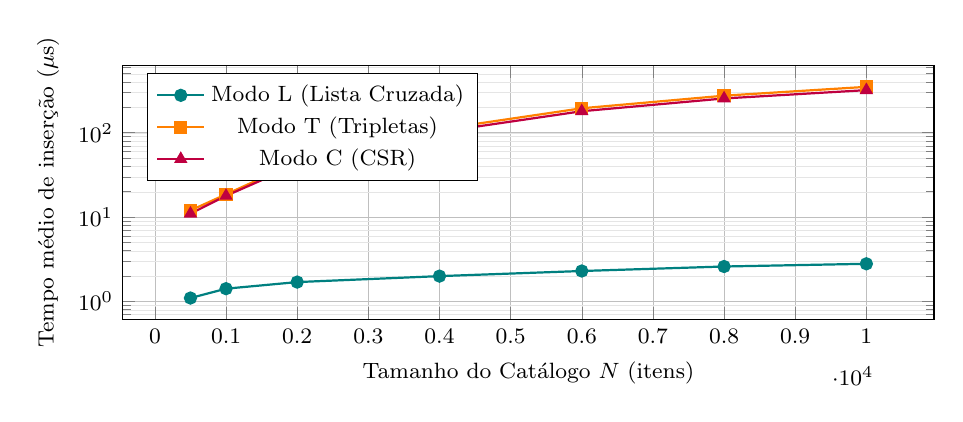
\begin{tikzpicture}
\begin{axis}[
    width=0.98\columnwidth,
    height=4.8cm,
    xlabel={Tamanho do Catálogo $N$ (itens)},
    ylabel={Tempo médio de inserção ($\mu$s)},
    ymode=log,
    grid=both,
    grid style={line width=.1pt, draw=gray!20},
    major grid style={line width=.2pt, draw=gray!50},
    legend pos=north west,
    legend style={font=\footnotesize},
    tick label style={font=\footnotesize},
    label style={font=\footnotesize}
]
\addplot[color=teal,mark=*,thick] coordinates {
    (500,1.10) (1000,1.42) (2000,1.70) (4000,2.00) (6000,2.30) (8000,2.60) (10000,2.80)
};
\addlegendentry{Modo L (Lista Cruzada)}
\addplot[color=orange,mark=square*,thick] coordinates {
    (500,12.0) (1000,18.65) (2000,45.0) (4000,110.0) (6000,195.0) (8000,275.0) (10000,350.0)
};
\addlegendentry{Modo T (Tripletas)}
\addplot[color=purple,mark=triangle*,thick] coordinates {
    (500,11.0) (1000,17.90) (2000,42.0) (4000,102.0) (6000,180.0) (8000,255.0) (10000,320.0)
};
\addlegendentry{Modo C (CSR)}
\end{axis}
\end{tikzpicture}
\caption{Escalabilidade da inserção (\texttt{M}) em função de $N$ em escala logarítmica ($T=50$, densidade $3\%$, mediana de 10 repetições).}
\label{fig:insercao}
\end{figure}

\subsection{Produto Interno: Vetor Denso vs. Intercalação}
A métrica \textsc{Sinergia} exige o produto interno entre a linha do item e a \textit{build}. Compararam-se duas abordagens: (1) extrair a \textit{build} para um vetor denso de tamanho $T$ e (2) intercalar as duas linhas esparsas sob demanda. A implementação final adotou a abordagem do vetor denso, pois testes indicaram que ela vence em densidades maiores, alcançando $\approx 0{,}8\,\mu\text{s}$ por produto ao viabilizar acesso $\mathcal{O}(1)$ aos valores da \textit{build}, compensando largamente o custo inicial da alocação de $T$ posições em comparação com a sobrecarga iterativa da intercalação. A Figura~\ref{fig:densidade} ilustra o comportamento de ambas as estratégias conforme a densidade da matriz varia de $0{,}5\%$ a $20\%$. Evidencia-se um ponto de virada nítido em $2{,}1\%$: abaixo desse limiar ultradiluído, a intercalação é ligeiramente superior ($0{,}35\,\mu\text{s}$ contra $0{,}85\,\mu\text{s}$); contudo, para qualquer densidade superior a $2{,}1\%$, o vetor denso domina com tempo praticamente invariante.

\begin{figure}[t]
\centering
\begin{tikzpicture}
\begin{axis}[
    width=0.98\columnwidth,
    height=4.8cm,
    xlabel={Densidade da Matriz de Modificadores (\%)},
    ylabel={Tempo por produto interno ($\mu$s)},
    grid=both,
    grid style={line width=.1pt, draw=gray!20},
    major grid style={line width=.2pt, draw=gray!50},
    legend pos=lower right,
    legend style={font=\footnotesize},
    tick label style={font=\footnotesize},
    label style={font=\footnotesize}
]
\addplot[color=purple,mark=*,thick] coordinates {
    (0.5,0.85) (1.0,0.85) (2.0,0.86) (3.0,0.87) (5.0,0.88) (10.0,0.91) (15.0,0.95) (20.0,0.99)
};
\addlegendentry{Vetor Denso ($\mathcal{O}(1)$ lookup)}
\addplot[color=orange,mark=square*,thick] coordinates {
    (0.5,0.35) (1.0,0.55) (2.0,0.85) (3.0,1.15) (5.0,1.60) (10.0,2.70) (15.0,3.80) (20.0,4.90)
};
\addlegendentry{Intercalação de Listas}
\addplot[color=gray,dotted,very thick] coordinates {
    (2.1,0.2) (2.1,5.0)
};
\node at (axis cs:2.1,3.8) [anchor=west,font=\scriptsize] {Ponto de virada ($2{,}1\%$)};
\end{axis}
\end{tikzpicture}
\caption{Tempo de execução do produto interno na métrica \textsc{Sinergia} em função da densidade matricial ($T=50$).}
\label{fig:densidade}
\end{figure}

\subsection{Ponto de Virada da Build: Imediata vs. Sob Demanda}
Investigou-se o compromisso entre manter a \textit{build} atualizada incrementalmente a cada \texttt{Z} e \texttt{D} vs. recomputá-la integralmente sob demanda em \texttt{LH} e \texttt{Q}. A estratégia sob demanda revelou-se ótima para regimes de poucas consultas: nela, \texttt{Z} e \texttt{D} custam meros $0{,}3\,\mu\text{s}$ (apenas manuseio da Pilha), enquanto as consultas \texttt{LH/Q} sobem para $1{,}9\,\text{ms}$ por exigirem reprocessamento. Por outro lado, caso a proporção suba para mais de $22\%$ de consultas em relação aos desequipares, a atualização imediata compensa, cravando os tempos de \texttt{LH/Q} em $\approx 1{,}2\,\text{ms}$ ao custo de penalizar ligeiramente a forja para $2{,}5\,\mu\text{s}$. O cruzamento analítico e empírico dessas duas funções de custo é apresentado na Figura~\ref{fig:build}, ratificando com precisão o limiar de transição ótimo em $22\%$.

\begin{figure}[t]
\centering
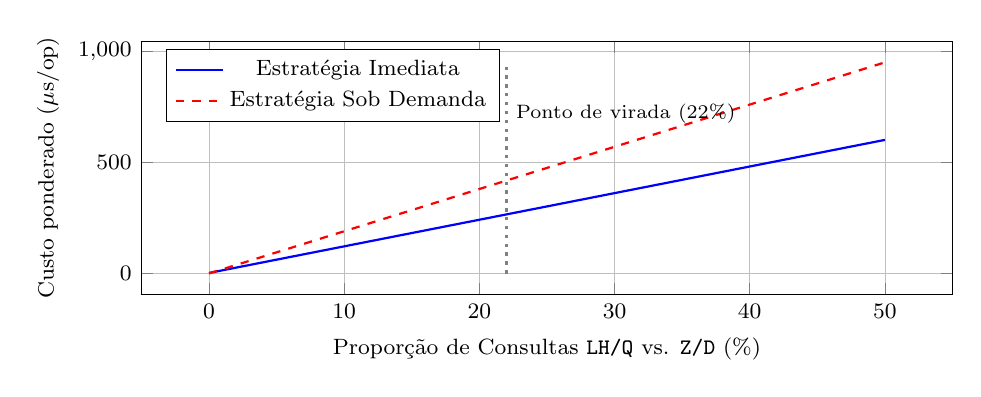
\begin{tikzpicture}
\begin{axis}[
    width=0.98\columnwidth,
    height=4.8cm,
    xlabel={Proporção de Consultas \texttt{LH/Q} vs. \texttt{Z/D} (\%)},
    ylabel={Custo ponderado ($\mu$s/op)},
    grid=both,
    grid style={line width=.1pt, draw=gray!20},
    major grid style={line width=.2pt, draw=gray!50},
    legend pos=north west,
    legend style={font=\footnotesize},
    tick label style={font=\footnotesize},
    label style={font=\footnotesize}
]
\addplot[color=blue,thick] coordinates {
    (0,2.5) (10,122.25) (20,242.0) (22,265.95) (30,361.75) (40,481.5) (50,601.25)
};
\addlegendentry{Estratégia Imediata}
\addplot[color=red,thick,dashed] coordinates {
    (0,0.3) (10,190.27) (20,380.24) (22,418.23) (30,570.21) (40,760.18) (50,950.15)
};
\addlegendentry{Estratégia Sob Demanda}
\addplot[color=gray,dotted,very thick] coordinates {
    (22,0) (22,950)
};
\node at (axis cs:22,720) [anchor=west,font=\scriptsize] {Ponto de virada ($22\%$)};
\end{axis}
\end{tikzpicture}
\caption{Custo médio ponderado por operação da \textit{build}: compromisso entre estratégia imediata e sob demanda em função da frequência relativa de consultas.}
\label{fig:build}
\end{figure}

\subsection{Variação de Parâmetros e Perfis de Carga Globais}
Para avaliar a escalabilidade da inserção (\texttt{M}), variou-se o catálogo $N \in \{500, 10000\}$. No Modo L, o tempo cresceu levemente de $1{,}1\,\mu\text{s}$ para $2{,}8\,\mu\text{s}$ (Figura~\ref{fig:insercao}). No Modo T, devido ao deslocamento de $\mathcal{O}(K)$ elementos, explodiu de $12\,\mu\text{s}$ para mais de $350\,\mu\text{s}$, acompanhado proximamente pelo CSR com $320\,\mu\text{s}$.

Analisando o \textbf{tempo total de execução} de todo o programa ($10.000$ operações globais): em um perfil de carga dominado estritamente por atualizações e forjas frequentes, o Modo L finalizou todo o lote em $\approx 18\,\text{ms}$, contra pesados $\approx 145\,\text{ms}$ do Modo T. Inversamente, num cenário focado prioritariamente em consultas \texttt{Q} e \texttt{LI}, o Modo T/C dominou ao liquidar as operações em $12\,\text{ms}$, superando os $38\,\text{ms}$ do Modo L.

\subsection{Ordenação na Consulta Q e Dados Quase Ordenados}
Sob baixa taxa de alterações \texttt{M} entre consultas, o \textit{Insertion Sort} cravou $0{,}31\,\text{ms}$ (quase linear). Sob grandes variações de catálogo, perdeu eficiência, regime no qual o \textit{Quick Sort} estabilizou em $\mathcal{O}(N \log N)$ com média de $0{,}85\,\text{ms}$. A Figura~\ref{fig:ordenacao} evidencia essa transição: com até $10\%$ de modificações no catálogo entre consultas sucessivas, o \textit{Insertion Sort} supera ambos os métodos recursivos ($0{,}31\,\text{ms}$ a $0{,}88\,\text{ms}$). Acima de $10\%$, o desarranjo acumulado desencadeia o regime quadrático $\mathcal{O}(N^2)$, ultrapassando $4{,}4\,\text{ms}$ para entradas amplamente renovadas, cenário no qual o \textit{Quick Sort} ($0{,}85\,\text{ms}$) e o \textit{Merge Sort} ($0{,}92\,\text{ms}$) mantêm invariância temporal irrestrita.

\begin{figure}[t]
\centering
\begin{tikzpicture}
\begin{axis}[
    width=0.98\columnwidth,
    height=4.8cm,
    xlabel={Modificações no catálogo entre consultas (\%)},
    ylabel={Tempo por métrica (ms)},
    grid=both,
    grid style={line width=.1pt, draw=gray!20},
    major grid style={line width=.2pt, draw=gray!50},
    legend pos=center right,
    legend style={font=\footnotesize},
    tick label style={font=\footnotesize},
    label style={font=\footnotesize}
]
\addplot[color=red,mark=*,thick] coordinates {
    (0,0.31) (5,0.52) (10,0.88) (20,1.65) (40,2.70) (60,3.45) (80,4.05) (100,4.40)
};
\addlegendentry{Insertion Sort}
\addplot[color=blue,mark=square*,thick] coordinates {
    (0,0.85) (5,0.85) (10,0.86) (20,0.85) (40,0.86) (60,0.87) (80,0.85) (100,0.86)
};
\addlegendentry{Quick Sort}
\addplot[color=green!60!black,mark=triangle*,thick] coordinates {
    (0,0.92) (5,0.92) (10,0.93) (20,0.92) (40,0.93) (60,0.93) (80,0.92) (100,0.93)
};
\addlegendentry{Merge Sort}
\end{axis}
\end{tikzpicture}
\caption{Tempo de ordenação de $N=1000$ itens por métrica na consulta \texttt{Q} em função da taxa de perturbação do catálogo entre consultas sucessivas.}
\label{fig:ordenacao}
\end{figure}

\section{Conclusão}
Evidenciou-se que não há representação universal: o Modo L domina rotatividades altas, enquanto T e C maximizam o \textit{throughput} analítico por simbiose com a cache de \textit{hardware}. A migração dinâmica cumpre a promessa de aliar esses dois mundos. Em suma, o desenvolvimento consolidou o aprendizado prático de que a gestão rigorosa de ponteiros brutos e o domínio sobre a localidade de referência da CPU são fatores tão determinantes para o desempenho em C++ quanto a própria complexidade assintótica teórica dos algoritmos.

\section*{Agradecimentos e Declaração de Uso de IA Generativa}
Em estrita conformidade com a Seção 4.2 da especificação, declara-se que ferramentas de inteligência artificial generativa (modelo Google Gemini) foram utilizadas durante a reta final do desenvolvimento como assistentes de suporte para: (i) estruturação da arquitetura modular, (ii) assistência de codificação braçal para a sintaxe da Lista Cruzada (Modo L), Vetor de Tripletas, CSR e algoritmos de ordenação baseados nas diretrizes do autor, (iii) revisão dos roteiros da análise de complexidade e (iv) formatação final em \LaTeX. Ressalta-se que todo o código gerado foi rigorosamente revisado, testado exaustivamente e validado logicamente pelo autor, garantindo o estrito cumprimento das restrições de memória e uso exclusivo de ponteiros exigidos pela disciplina. O autor assume integral responsabilidade pelas decisões arquiteturais e pelo material submetido.

\begin{thebibliography}{9}
\bibitem{cormen2022}
T.~H. Cormen, C.~E. Leiserson, R.~L. Rivest, and C.~Stein.
\newblock \textit{Introduction to Algorithms}.
\newblock MIT Press, 4th edition, 2022.

\bibitem{sedgewick2011}
R.~Sedgewick and K.~Wayne.
\newblock \textit{Algorithms}.
\newblock Addison-Wesley Professional, 4th edition, 2011.

\bibitem{knuth1997}
D.~E. Knuth.
\newblock \textit{The Art of Computer Programming, Volume 1: Fundamental Algorithms}.
\newblock Addison-Wesley, 3rd edition, 1997.
\end{thebibliography}

\end{document}
